\chapter{Simulation study}
To verify that the FHTBoost algorithm developed works, we need to test it on simulated data.
As \citet{simulation-studies} say, there are several ways to use simulation studies.
In this chapter we describe two scenarios, a highly correlated scenario and an uncorrelated scenario. 
For each scenario, we estimate parameters based on the FHTBoost algorithm, and assess its performance.
The scenarios are both thought to be realistic scenarios where one has clinical measurements, in a high-dimensional covariate matrix $\X$, as well as gene expressions,
in a low-dimensional covariate matrix $\Z$.
We link each covariate to a parameter in a parameter vector, where $\X$ corresponds to $\bbeta$, and $\Z$ corresponds to $\bgamma$.
In each parameter vector, we set a small number of parameters to a non-zero value, and all the rest to zero.
This means that only a very small number of covariates have an effect.
Given these parameter vectors and covariate matrices, we can calculate a specific $y_0$ and a $\mu$ for each individual.
Based on these parameters, we can draw an observation from the inverse Gaussian distribution, which is then a realization of a lifetime based on the first-hitting time framework with a Wiener process.

In addition to verifying that the algorithm works, i.e., has predictive power and selects correct variables, we wish to see which of the two versions of the algorithm works best.
The fixed intercept version or the changing intercept version.

As discussed previously, it is important to have a separate and unseen test set.
Each training set will be generated by drawing $N=500$ individuals as described above, with a specific seed.
Since we are simulating, it is simple to generate a test set by drawing from a unique seed.
We are therefore also able to make the test set quite large, and larger than the training sets, with $N_{\text{test}}=1000$ observations.

We generate $B\approx500$ data sets by drawing according to algorithm X. Each data set has $N=500$ observations. 
We treat each data set as a separate training data set, and thus estimate $B$ models.
To estimate each model, we first perform repeated 5-fold cross validations, with 5 repeats, on the training data set.
As shown in section ..., this should provide a reasonably stable $\mstop$ (near the ``true'' $\mstop$) for that specific data set.
We then estimate a model on the test set, by running FHTBoost with $\mstop$ number of iterations.
The boosting algorithm has two main purposes: Selection of variables, and minimizing test error.
To assess variable selection, we look at some classification metric.
To assess test error, we calculate the difference of deviance on the test set.
We first discuss these metrics.

\section{Variable selection metrics}
As shown in section \eqref{sec:variable-selection}, a component-wise gradient boosting algorithm, such as FHTBoost,
performs data-driven variable selection.
We wish to see how FHTBoost performs with regard to selecting variables which we have specified to be informative.

In a given estimated boosting model, the model has selected a certain amount of variables.
We denote a selected variable as a ``positive,'' or $P$ for short, and a variable which is not selected as ``negative'', or $N$ for short.
Since we know which variables actually affect the response, we know how many of the variables selected are selected correctly, in the sense
that they are selected and they have an effect. We call these true positives, or $TP$ for short.
Similarly, we know which variables do not affect the response, and so we can calculate the number of non-informative variables
which were not selected, i.e., true negative, or $TN$ for short. Furthermore, we say that variables which have been selected
but which do not actually have an effect, are false positives, $FP$. Finally, false negatives, $FN$, are variables which do actually
have an effect, but which were not selected in the boosting model.

\subsection{Sensitivity}
Ideally, this is 1.
\begin{equation}\label{eq:sensitivity}
    \text{Sensitivity}=\frac{TP}{P}
\end{equation}

\subsection{Specificity}
Ideally, this is 1.
\begin{equation}\label{eq:specificity}
    \text{Specificity}=\frac{TN}{N}
\end{equation}

\subsection{False prediction rate}
Ideally, this is 0.
\begin{equation}\label{eq:accuracy}
    \text{FPR}=\frac{FP}{FP+TP}
\end{equation}


\subsection{Accuracy}
Ideally, this is 1.
\begin{equation}\label{eq:accuracy}
    \text{ACC}=\frac{TP+TN}{P+N}
\end{equation}
Accuracy is a common metric to use when considering classification of something. However, in our case, we have very imbalanced classes. We have very few positive labels, i.e., parameters which are non-zero in the true parameter vector, which we called $P$. Therefore the denominator above, $P+N$ will be dominated by the very large $N$ number. Since a properly tuned boosting algorithm will do early stopping, we will end up with a model which has a small number of chosen parameters. Therefore, inevitably, our $TN$ will be very large, simply because there are a lot of negatives, and we just don't even have the time to choose them. Therefore we conclude by not using accuracy to evaluate our model.

\subsection{Difference in deviance}
Difference in deviance is a measurement for comparing models of the same type, e.g., between different parameter vectors of an FHT model.
The objective of the measurement is to assess how much the model improves when adding covariates.
When estimating the FHT model, we first find the intercepts of the covariate vectors, $\beta_0$ and $\gamma_0$, respectively,
and the initial covariate vectors, i.e., the covariate vectors before starting boosting, are
\begin{equation*}
    \bbeta^{[0]}=(\beta_0^{[0]},0,0,\ldots,0)
\end{equation*}
and
\begin{equation*}
    \bgamma^{[0]}=(\gamma_0^{[0]},0,0,\ldots,0)
\end{equation*}
We denote the concatened vector of these as
\begin{equation*}
    \btheta^{[0]}=\left(\bbeta^{[0]},\bgamma^{[0]}\right).
\end{equation*}
We call this the \textit{null model}.
Similarly, the fully estimated covariate vectors, boosted with $\mstop$ steps, on the training set, are
\begin{equation*}
    \bbeta^{[\mstop]}_{\text{train}}=(\beta_0^{[\mstop]},\beta_1^{[\mstop]},\beta_2^{[\mstop]},\ldots,\beta_p^{[\mstop]})
\end{equation*}
and
\begin{equation*}
    \bgamma^{[\mstop]}_{\text{train}}=(\gamma_0^{[\mstop]},\gamma_1^{[\mstop]},\gamma_2^{[\mstop]},\ldots,\gamma_d^{[\mstop]}).
\end{equation*}
Again let their concatenation be denoted as
\begin{equation*}
    \btheta^{[\mstop]}_{\text{train}}=\left(\bbeta^{[\mstop]}_{\text{train}},\bgamma^{[\mstop]}_{\text{train}}\right).
\end{equation*}
We call this the model.
The deviance of a model $\btheta$ is
\begin{equation}
    \text{dev}(\btheta)=2l(\btheta),
\end{equation}
where $l(\btheta)$ is the log-likelihood value attained by an estimated covariate vector $\btheta$.
The difference of deviance between two models $\btheta_1$ and $\btheta_2$ is
\begin{equation}
    d=\text{dev}(\btheta_1)-\text{dev}(\btheta_2)=2l(\btheta_1)-2l(\btheta_2)=2\left(l(\btheta_1)-l(\btheta_2)\right).
\end{equation}
In our case, the null model, without covariates, is a boosted model with zero iterations, i.e., a model with only the intercepts, and its likelihood is given by
\begin{equation}
    l^{\text{test}}\left(\btheta^{[0]}_{\text{train}}\right).
\end{equation}
The notation here tries to make the point that the covariate vector is estimated on the \textit{training} set, and the log-likelihood value is calculated on the \textit{test} set.
Further, the trained model, with covariates, is a model $\btheta^{[\mstop]}_{\text{train}}$, i.e., a model boosted with $\mstop$ steps.
The estimated model has a likelihood of
\begin{equation}
    l^{\text{test}}\left(\btheta^{[\mstop]}_{\text{train}}\right).
\end{equation}
It is conventional to put the least complex model first, and the more complex model last.
Since a more complex model should achieve a better, and thus higher, log-likelihood, the difference of deviance should be negative. 
Hence the difference in deviance between a fitted model and the null model containing no covariates is
\begin{equation*}
    d=2\left(l^{\text{test}}\left(\btheta^{[0]}_{\text{train}}\right)-l^{\text{test}}\left(\btheta^{[\mstop]}_{\text{train}}\right)\right).
\end{equation*}
The performance of a model is good when $d$ is small, meaning ``very negative.''
In some of the results in this section, we end up with a \textit{positive} difference of deviance.
This means that the null model achieved a higher log-likelihood value than the fully estimated model.
This might happen if the model estimated on the training set has estimated parameters which are in the opposite direction of those in the test set.

\section{Simulation of survival data from an IG FHT distribution}\label{sec:simulate-IG-data}
We wish to simulate survival times $\ti,i=1,\ldots,n$ with censoring. We first draw $n$ (uncensored) survival times $\tilde{t}_i$ from some survival time distribution $f(\cdot)$. If this distribution has a closed form probability distribution function, we can draw from it directly. If not, we may use an inverse sampling method, e.g. by drawing unit exponentials and using a corresponding transformation.

To censor the data, we draw censoring times $W_i\sim f(\cdot),i=1,\ldots,N$, from a more right-tailed distribution, meaning we want to get many, but not all, $W_i$'s to be larger than the $\tilde{t}_i$'s. We let the observed survival times then be $t_i=\min(\tilde{t}_i,W_i)$.
The corresponding observed indicator, $d_i$, is then set equal to 1 if the actual survival time was observed, i.e., if $\ti<W_i$. We end up with a set of $N$ tuples $(t_i,d_i),i=1,\ldots,N$. Note that this scheme incorporates independent censoring: The censoring time is independent of the survival times.

\begin{algorithm}
\caption{Generating survival data from Inverse Gaussian FHT distribution}
\label{algo:FHT-sim}
\begin{enumerate}
    \item Given design matrices $\X$, $\Z$ and true parameter vectors $\bbeta$ and $\bgamma$.
    \item Specify censoring time distribution.
    \item Calculate distribution parameters $y_0$ and $\mu$ using link functions,
        \begin{align*}
            y_0&=\exp(\bbeta^T\X) \\
            \mu&=\bgamma^T\Z.
        \end{align*}
    \item Draw $N$ uncensored survival times $(\tilde{t}_i)_{i=1}^N$ from IG$(\mu,y_0)$.
    \item Draw $n$ censoring times $W_1,W_2,\ldots,W_n$ from a censoring time distribution which is independent of the data.
    \item Right censor the survival times by choosing $t_i=\min(\tilde{t}_i,W)$.
        The indicator on whether observation $i$ was observed or not is then $\delta_i=I(t_i=\tilde{t}_i)$.
    \item The simulated data set is $D=(t_i,\,d_i)_{i=1}^N$.
\end{enumerate}
\end{algorithm}

\section{Generating correlated clinical and gene expression data}
To create a realistic scenario where we have data looking like gene expression data and clinical data, we need an algorithm.
In very broad terms, this is an algorithm for setting up a correlation structure (via a covariate matrix) and then drawing covariate matrices from a
normal distribution.

We imagine a scenario where we for each individual have a covariate matrix $X$ consisting of $p_1$ gene expressions, and a
covariate matrix $Z$ consisting of $p_2$ clinical measurements.
We can imagine that some of the genes in $X$ are highly correlated. One way to imagine this is to imagine that we have blocks of genes,
where inside one block, the genes are highly correlated, whereas genes in one block are not correlated to other genes.
In addition, one block of genes might affect a block of clinical variables as well.

We specify a number of blocks $B$. A given block $b,b=1,2,\ldots,B$, contains a certain number of genes, $G_b$, which are correlated to each other.
It also contains a certain number of clinical measurements, $C_b$. These measurements are correlated to each other, and to the genes in the block.

After setting up the block structure, we 

There are three types of correlations.
1. Within each block of genes. Defaults to 0 for genes not belonging to any block.
2. Between clinical predictors in each pathway
3. Between the clinical and molecular predictors in each pathway


\section{Simulation setup}
We do simulations where we draw observations from the Inverse Gaussian distribution, i.e., we simulate lifetimes from the first hitting time model with Wiener process as the health process. We use algorithm \eqref{algo:FHT-sim} to do this. We will have two scenarios: One with no correlation, and one with a lot of correlation. To simulate the covariate matrices $X$ and $Z$ we will use algorithm \eqref{algo:clinical-sim}, which is a method for simulating clinical and gene data together. We imagine $X$, corresponding to $\bbeta$, be gene expressions, whereas $Z$, corresponding to $\bgamma$ be clinical measurements. We specify the different correlations for the covariate matrices. But most importantly, we specify the true parameter vectors, $\bbeta$ and $\bgamma$. For each scenario, we conduct $N_{\text{scenario}}$ runs.

One run consists of first drawing data (with a specific seed to ensure reproducibility), i.e., we draw covariate matrices $\X$, $\Z$ from \label{algo:clinical-sim}. $\X$ is of size $n\times p$ and $\Z$ is of size $n\times d$, where $n$ is the number of observations, $p+1$ is the size of the covariate vector $\bbeta$ (including an intercept which will not be affected by the covariates), and $d+1$ is the size of the covariate vector $\bgamma$. Then we combine these with the true covariate matrices to get vectors $\y_0$ and $\mathbf{\mu}$ of initial value of the health process, and drift, respectively. Then we draw from the Inverse Gaussian distribution according to \label{algo:FHT-sim}, obtaining $n$ right-censored lifetimes, i.e., $n$ tuples $(t_i,d_i)_{i=1,\ldots,N}$. With these tuples, then, we can do a run with the FHT boosting algorithm. We first use repeated K-fold cross-validation to find the optimal number of boosting steps, $m_{\text{stop}}$. Then we estimate the model on the whole of this training set. Then we validate this model on a training set of size $N_{\text{test}}$. The data here is drawn in the exact same manner as the training data, here also with a specific seed.

\begin{algorithm}
\caption{Generating correlated clinical and gene expression data}
\label{algo:clinical-sim}
\begin{enumerate}
    \item Lorem ipsum.
\end{enumerate}
\end{algorithm}

\section{Large simulation with uncorrelated matrices}
Here, $N$ is 500. We let $\bbeta$ be a large vector of size $p=10001$, and $\bgamma$ be a small vector of size $d=16$. Specifically, we set the intercept term in $\bbeta$ to be 2.0, and the first 35 elements to be 0.1. We set the rest to be 0. For $\bgamma$, we set the intercept term to be -1, and in similar fashion, let the first 5 elements have a non-zero value of -0.1. Here also we set the remaining 10 elements to be 0.
Hence, the true parameter vectors are as follows:
\begin{align*}
    \bbeta=\left(2.0, \underbrace{0.1, 0.1, \ldots, 0.1}_{\text{length 35}}, \overbrace{0, 0, \ldots, 0}^{\text{length 9965}}\right) \\
    \bgamma=\left(-1.0, \underbrace{0.1, 0.1, \ldots, 0.1}_{\text{length 5}}, \overbrace{0, 0, \ldots, 0}^{\text{length 10}}\right)
\end{align*}
We draw $X$ and $Z$ from the algorithm for drawing clinical and gene data, with $B=0$ blocks.

Choosing 0.1 for the informative parameter effects $\beta_j,j=1,2,\ldots,35$, might seem like it is too low.
The parameter vector $\bbeta$ is linked to the initial level $y_0$ by an exponential link function.
This means that each parameter effect is multiplicative instead of additive.
A large gene expression value here can potentially cause a large change in $y_0$, and especially if there are several rather extreme values.
With 35 genes that do affect $y_0$, the chance of having one or several large gene values is rather large.
Although we do standardize before drawing.
Because of this, I had trouble setting up any simulation in which the algorithm managed to pick up much of the underlying parameter vector.
That is why the true parameter effects are rather small.
In retrospect, the parameter effects for the drift $\mu$ could have been larger.
One reason being that in this setup the effects of a unit increase in a gene is $\exp(0.1)=1.1$, and so an effect of only 0.1 on the drift is rather small in comparison.
Another reason is that we hypothesize that a clinical measurement should have more effect than a gene.

We specify that all correlations are 0, meaning no covariate correlates with any other.

With this exact setup, we run a simulation experiment $B=500$ times, where we at the beginning of each simulation set the seed, via \verb|set.seed(seed)| to be $b=1,\ldots,B$.
We first generate matrices $X$ and $Z$, and simulate FHT times from the algorithm above.
We then run cross validation on this data set to find the optimal iteration number $m_{\text{stop}}$.
Below is a box plot of the resulting times. We then run a boosting algorithm with $m_{\text{stop}}$ steps on the training set, and use the resulting model on the test set.

\subsection{Boosting with changing the intercept}
See Table \ref{table:non-correlated-with-intercept-summary}, Table \ref{table:non-correlated-with-intercept-y0}, and \ref{table:non-correlated-with-intercept-mu}.
\begin{table}\caption{Summary of results with intercept boosting}\label{table:non-correlated-with-intercept-summary}
\centering
\begin{tabular}{lccccc}
\toprule
Measure &   Mean & Standard error &  Minimum &    Maximum & Median \\
\hline
$d$    &    -92.0 & 41.8 &  -233.6   &  7.2 &  -91.4 \\
$\mstop$      &    15.8 &  6.4 &     2 &    39 & 16.0\\
%$l^{\text{test}}\left(\bbeta^{[\mstop]}_{\text{train}}\right)$      & -2325.7 & 20.4 & -2382.8 & -2270.0 & -2326.9\\
%$l^{\text{test}}\left(\bbeta^{[0]}_{\text{train}}\right)$ & -2371.7 &  3.9 & -2396.8 & -2368.8 &-2370.4
\bottomrule
\end{tabular}
\end{table}

\begin{table}\caption{Variable selection results on $y_0$, $\beta$, uncorrelated scenario, with changing intercept}\label{table:non-correlated-with-intercept-y0}
\centering
\begin{tabular}{lccc}
\toprule
Measure &  Mean & Median & Standard error \\
\hline
Sensitivity & 0.190 &  0.171 & 0.090 \\
Specificity & 1.000 &  1.000 & 0.000 \\
False discovery rate & 0.310 &  0.333 & 0.176 \\
\bottomrule
\end{tabular}
\end{table}


\begin{table}\caption{Variable selection results on $\mu$, $\gamma$, uncorrelated scenario, with changing intercept}
\centering
\begin{tabular}{lccc}
\toprule
Measure     & Mean  & Median & Standard error     \\
\hline
Sensitivity & 0.741 &  0.800 & 0.232 \\
Specificity & 0.943 &  1.000 & 0.110 \\
False discovery rate & 0.091 &  0.000 & 0.144 \\
\bottomrule
\end{tabular}
\end{table}



\subsection{Boosting \textit{without} changing the intercept}
See Table \ref{table:non-correlated-no-intercept-summary}, Table \ref{table:non-correlated-no-intercept-y0}, and \ref{table:non-correlated-no-intercept-mu}.
\begin{table}\caption{Summary of results without intercept boosting}\label{table:non-correlated-no-intercept-summary}
\centering
\begin{tabular}{lccccc}
\toprule
Measure &    Mean &     Standard error &  Minimum & Maximum & Median \\
\hline
$d$    &   -130.1 & 40.7 &   -255.2   &   -5.7 & 131.0 \\
$\mstop$      &    63.8 & 26.5 &     2 &   160 & 67.5 \\
%$l^{\text{test}}\left(\bbeta^{[\mstop]}_{\text{train}}\right)$   & -2306.7 & 21.5 & -2370.6 & -2241.7 &-2305.2\\
%$l^{\text{test}}\left(\bbeta^{[0]}_{\text{train}}\right)$ & -2371.7 &  3.9 & -2396.8 & -2368.8&-2370.4
\bottomrule
\end{tabular}
\end{table}

\begin{table}\caption{Variable selection results on $y_0$, $\beta$, uncorrelated scenario, with fixed intercept}
\label{table:non-correlated-no-intercept-y0}
\centering
\begin{tabular}{lccc}
\toprule
Measure &  Mean &  Median &   Standard error \\
\hline
Sensitivity & 0.452 &  0.457 & 0.162 \\
Specificity & 0.997 &  0.997 & 0.002 \\
False discovery rate & 0.584 &  0.613 & 0.144 \\
\bottomrule
\end{tabular}
\end{table}


\begin{table}\caption{Variable selection results on $\mu$, $\gamma$, uncorrelated scenario, with fixed intercept}\label{table:non-correlated-no-intercept-mu}
\centering
\begin{tabular}{lccc}
\toprule
Measure &  Mean & Median & Standard error \\
\hline
Sensitivity & 0.958 &  1.000 & 0.099 \\
Specificity & 0.638 &  0.700 & 0.291 \\
False discovery rate & 0.365 &  0.375 & 0.192 \\
\bottomrule
\end{tabular}
\end{table}

\begin{figure}\label{fig:simulation-not-correlated-deviances-boxplot}
\caption{Boxplot for difference in deviance for the two intercept variants, non-correlated scenario}
\centering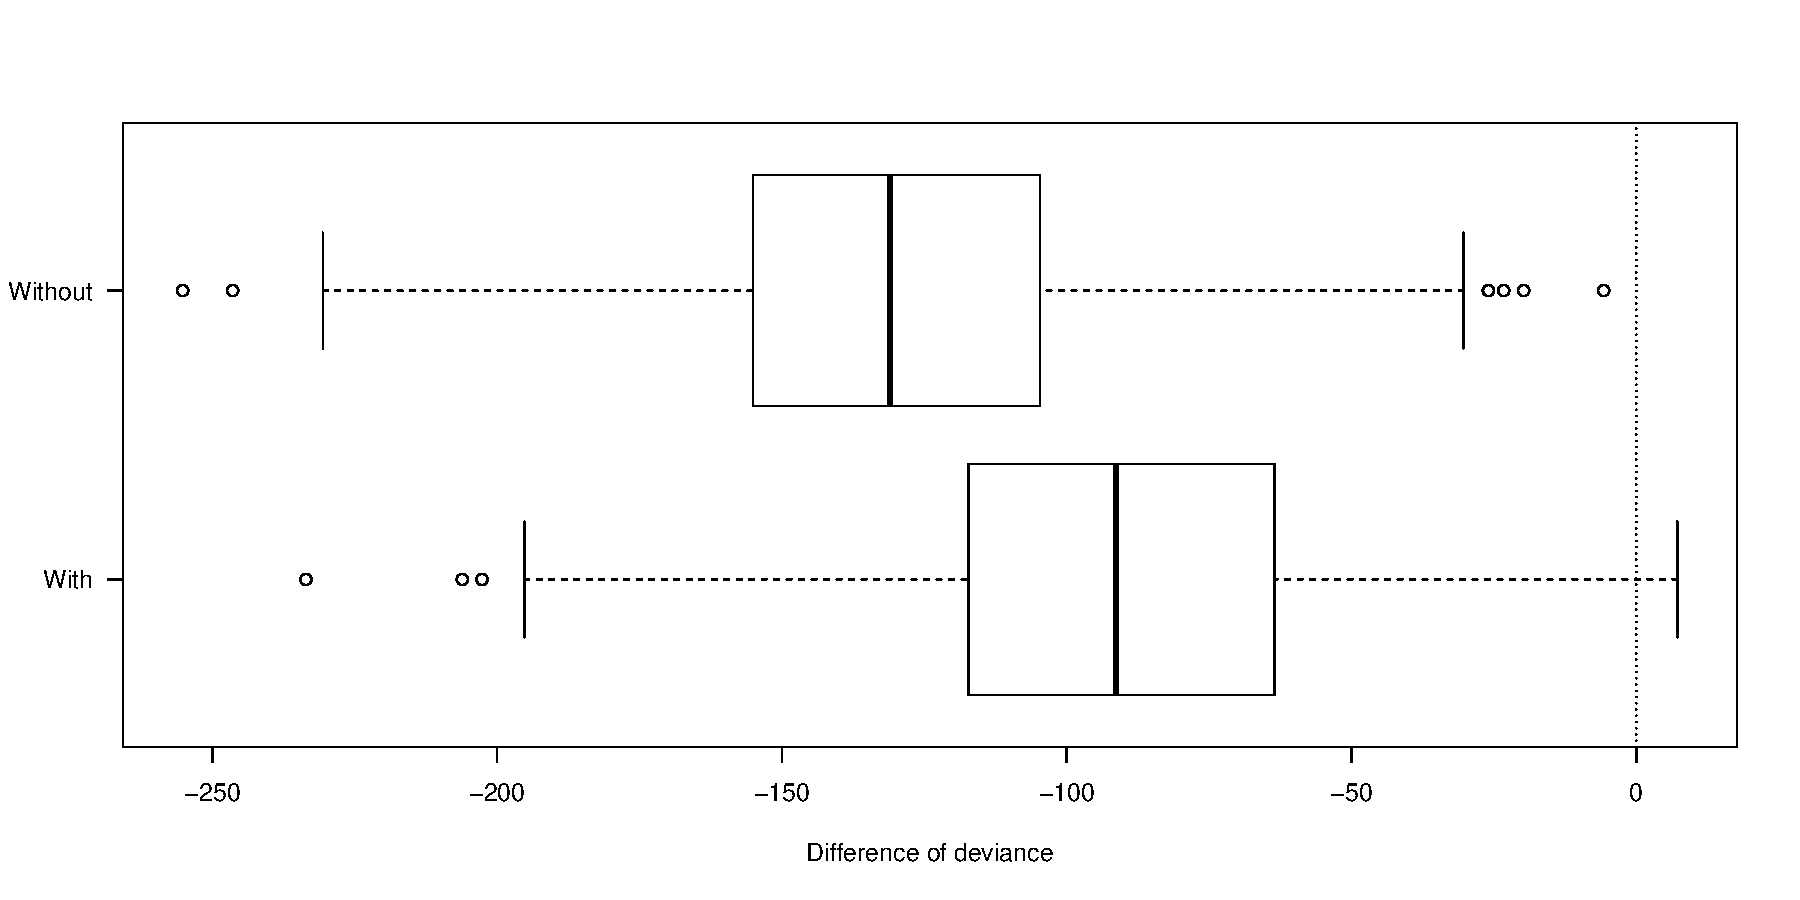
\includegraphics[scale=0.4]{deviances_simulation.pdf}
\end{figure}

\subsection{Thoughts}
Note first that the two versions of the algorithm have very different $\mstop$ values.
The stopping iteration $\mstop$ when continuously changing the intercept is quite lower than when boosting without.
This means that the resulting covariates for the intercept version are more shrunken than for the no intercept version.
This suggests that the non-fixed intercept version is quicker to overfit, since the $\mstop$ should find approximately the iteration number which minimizes overfitting.
Since the covariate vector is estimated on the training data, a likely explanation is that the changing intercept captures more of the variation in the training data.
In doing so, there is less variation to be explained by the covariates, and hence the boosting algorithm will start to overfit more quickly.
We see that the median difference of deviance on the intercept version is -91.955, while it is -130.109 on the non-intercept version.
We should therefore conclude that the non-intercept version is better, if we want to choose between the two.
Look at the boxplot in figure \ref{fig:simulation-not-correlated-deviances-boxplot}.
Another thing to note here is that the fixed intercept version has no occurrence of a positive difference of deviance.
In other words, all estimated models performed better than their null models.

We further look at the variable selection metrics.
These are organized by covariate vector.
In each run, we counted $TP$, the number of informative covariates which were selected in the estimated boosting model.
We similarly counted $TN$, the number of non-informative covariates which were selected in the model.
Our setup has as many as 35 informative gene covariates and 5 informative clinical covariates.
Since the no-intercept version has a rather low number of iterations, with a median of 16, it is impossible to get anywhere near perfect on these metrics, as at most one new parameter is selected in each iteration.

Furthermore, we are considering the sensitivity and specificity on both covariate vectors at the same time.
This means that these scores will affect each other.

Consider first the result of the version in which the intercept is changed in each step.
Both covariate vectors have a very high specificity, which measures the amount of negatives which are correctly classified as negatives.
In both cases, these are almost 1.
In fact, for $\bbeta$, although it is not exactly 1, but rather 0.999667937538074.
When rounded to 3 significant digits, this is 1, and similarly, the standard error rounded is 0.000.
Keep in mind here that the denominator in these cases is 9965.
If we only look at $FN$, i.e., false positives, which is $N-TN$, the mean is 3.31, with a standard error of 2.50.
With a median false discovery rate of 0.333, there is a one in three chance that we select a variable which is not actually informative.
The sensitivity, i.e., the ratio of correctly selected informative variables, has a median of only 0.171.
This means that a large proportion of the informative covariates are not selected.
As we alluded to earlier, this is to be expected due to a low number of iterations.
For $\bgamma$, a much higher specificity is attained, with a median at 0.800.
Even though the parameter effects on the drift are rather small, the informative covariates are often correctly selected.
Furthermore, the false discovery rate here is very low, with a median at 0.000.

Now consider the results of the fixed intercept version.
For the $\bbeta$ covariate vector, a higher proportion of informative covariates are selected, with a median sensitivity of 0.457.
Simultaneously, a larger false discovery rate of 0.584 is not good.
At the same time, the $\bgamma$ covariate vector has a really good sensitivity, with a median of 1, and a good specificity with a median of 0.700.
The false discovery rate on $\bgamma$ is slightly above one in three, with a median of 0.375.

\section{Large simulation with correlated matrices}
\subsection{Setup}
Lorem ipsum dolor sit amet.
Lorem ipsum dolor sit amet.
Lorem ipsum dolor sit amet.
Lorem ipsum dolor sit amet.
Lorem ipsum dolor sit amet.
Lorem ipsum dolor sit amet.
Lorem ipsum dolor sit amet.
Lorem ipsum dolor sit amet.
Lorem ipsum dolor sit amet.
Lorem ipsum dolor sit amet.
Lorem ipsum dolor sit amet.

\subsection{Boosting with changing the intercept}
See table \ref{table:correlated-intercept-summary}, table \ref{table:correlated-intercept-y0}, and \ref{table:correlated-intercept-mu}.
\begin{table}\caption{Summary of results with intercept boosting}\label{table:correlated-intercept-summary}
\begin{tabular}{lccccc}
Measure &    Mean &    Standard error &  Minimum & Maximum & Median \\
\hline
$d$    &    -57.8 & 47.2 &   -203.4 & 87.6 & -53.6 \\
$\mstop$      &    20.0 & 12.1 &     2 &    65 &  19.5 %\\
%$l^{\text{test}}\left(\bbeta^{[\mstop]}_{\text{train}}\right)$ & -2230.5 & 25.8 & -2342.6 & -2161.7 & -2230.3\\
%$l^{\text{test}}\left(\bbeta^{[0]}_{\text{train}}\right)$ & -2259.4 & 13.4 & -2350.8 & -2250.0 & -2254.6
\end{tabular}
\end{table}

\begin{table}
\caption{Variable selection results on $y_0$, $\beta$, correlated scenario, with changing intercept.}
\label{table:correlated-intercept-y0}
\centering
\begin{tabular}{lccc}
\toprule
Measure &  Mean &  Median &  Standard error \\
\hline
Sensitivity & 0.157 &    0.143 & 0.084 \\
Specificity & 0.999 &    0.999 & 0.000 \\
False discovery rate & 0.439 & 0.500 & 0.218 \\
\bottomrule
\end{tabular}
\end{table}

\begin{table}
\caption{Variable selection results on $\mu$, $\gamma$, correlated scenario, with changing intercept.}
\label{table:correlated-intercept-mu}
\centering
\begin{tabular}{lccc}
\toprule
Measure     & Mean & Median   & Standard error     \\
\hline
Sensitivity &  0.273 &  0.200 & 0.187 \\
Specificity &  0.831 &  0.867 & 0.139 \\
False discovery rate &  0.454 &  0.500 & 0.250 \\
\bottomrule
\end{tabular}
\end{table}

\subsection{Boosting \textit{without} changing the intercept}
See table \ref{table:correlated-no-intercept-summary}, table \ref{table:correlated-no-intercept-y0}, and \ref{table:correlated-no-intercept-mu}.
\begin{table}
\caption{Summary of results without intercept boosting}
\label{table:correlated-no-intercept-summary}
\centering
\begin{tabular}{lccccc}
\toprule
Measure &    Mean &     Standard error &  Minimum & Maximum & Median \\
\hline
$d$    &    -58.8 & 46.1 &  -223.1  &   73.5 & -54.5 \\
$\mstop$      &    51.1 & 24.4 &     2 &   148 & 50 \\
%$l^{\text{test}}\left(\bbeta^{[\mstop]}_{\text{train}}\right)$   & -2230.0 & 30.3 & -2351.3 & -2159.6 & -2228.4 \\
%$l^{\text{test}}\left(\bbeta^{[0]}_{\text{train}}\right)$ & -2259.4 & 13.4 & -2350.8 & -2250.0 & -2254.6
\bottomrule
\end{tabular}
\end{table}

\begin{table}
\caption{Variable selection results on $y_0$, $\beta$, correlated scenario, with fixed intercept.}
\label{table:correlated-no-intercept-y0}
\centering
\begin{tabular}{lccc}
\toprule
Measure &  Mean & Median &   Standard error \\
\hline
Sensitivity &    0.204 &    0.200 &  0.081 \\
Specificity &    0.998 &    0.998 &  0.001 \\
False discovery rate & 0.652 &    0.690 &  0.181 \\
\bottomrule
\end{tabular}
\end{table}


\begin{table}
\caption{Variable selection results on $\mu$, $\gamma$, correlated scenario, with fixed intercept.}
\label{table:correlated-no-intercept-mu}
\centering
\begin{tabular}{lccc}
\toprule
Measure     & Mean &Median  & Standard error     \\
\hline
Sensitivity & 0.625 &  0.700 & 0.245 \\
Specificity & 0.537 &  0.533 & 0.236 \\
False discovery rate         & 0.507 &  0.500 & 0.130 \\
\bottomrule
\end{tabular}
\end{table}

\begin{figure}
\caption{Boxplot for difference in deviance for the two intercept variants, non-correlated scenario}
\label{fig:simulation-not-correlated-deviances-boxplot}
\centering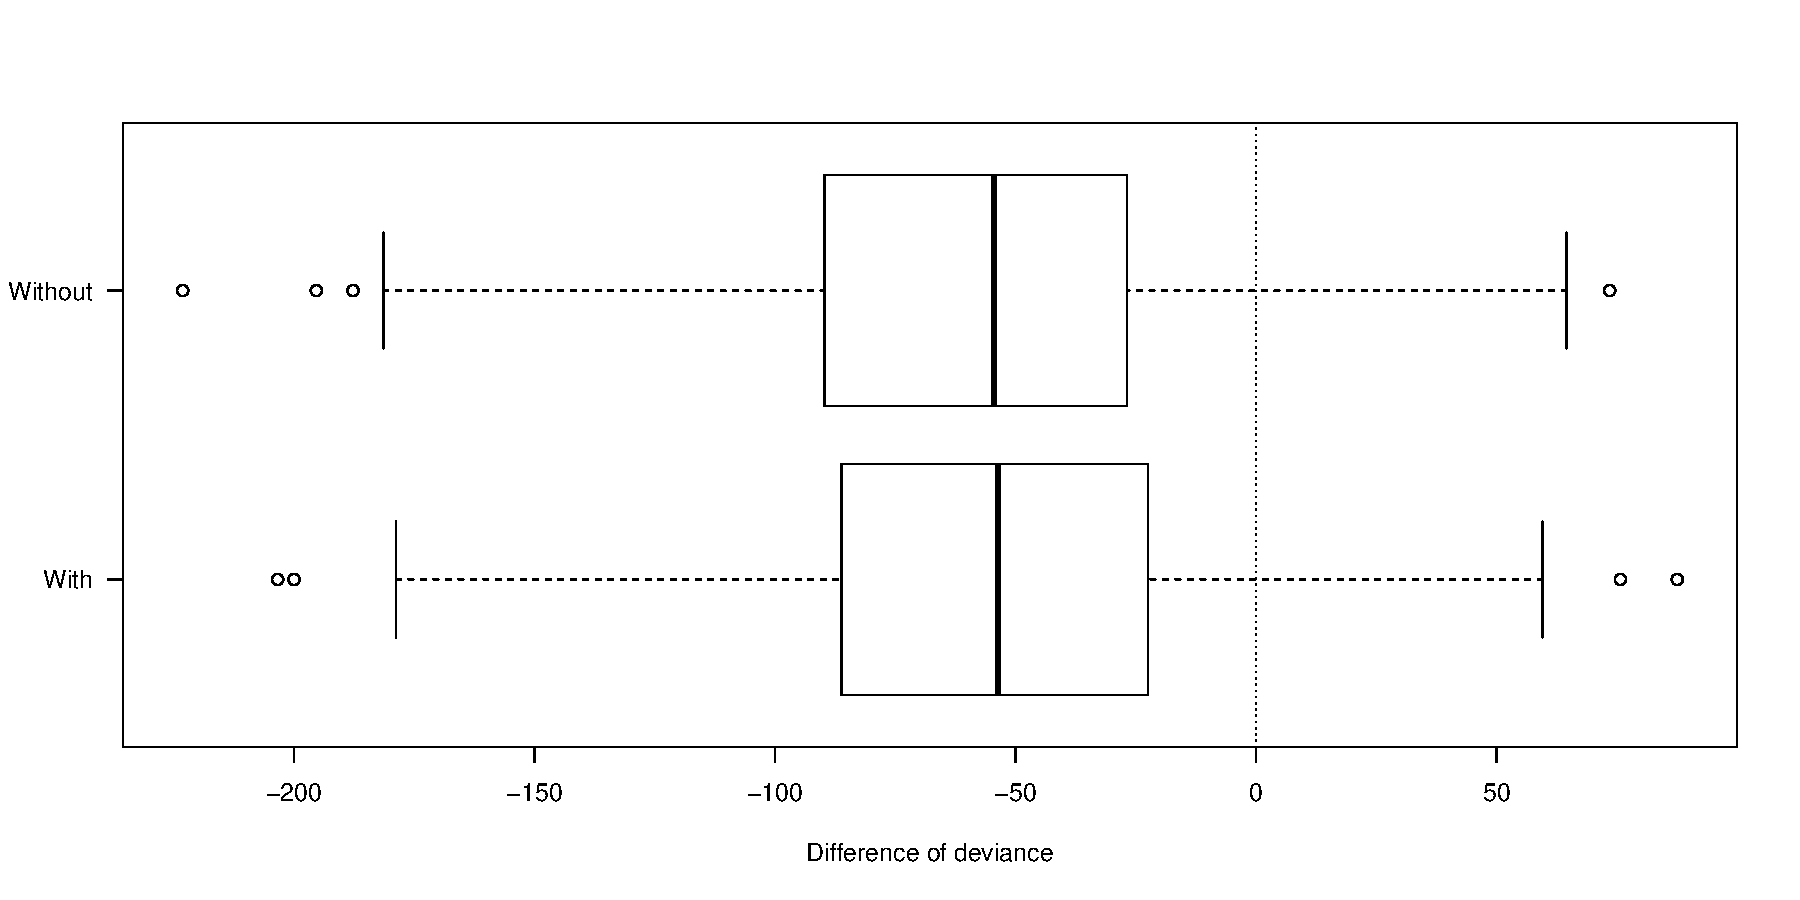
\includegraphics[scale=0.4]{deviances_simulation_correlated.pdf}
\end{figure}


\subsection{Thoughts}
For this scenario, as well, we see that the fixed intercept version has a higher optimal iteration number $\mstop$, a median of 50, compared to a median of 19.5 for the changing intercept version.
Again this necessarily means that more variables are selected.
We see that the median deviance is very slightly better for the fixed intercept version, and with better extreme values, both minimum and maximum.
See Figure \ref{fig:simulation-not-correlated-deviances-boxplot} for a boxplot of the difference of deviance for the two versions.

Now consider the variable selection metrics.
We first look at the covariate vector $\bbeta$, which affects the initial level $y_0$.
The fixed intercept version is slightly better with regards to sensitivity, i.e., selecting informative variables, with a median of 0.200 versus a median of 0.143 for the changing intercept version.
This does come at a cost of a higher false discovery rate, with a median of 0.690, where the changing intercept version has a median of 0.500.
In both versions, then, it is at least as likely to select a non-informative variable as an informative variable.
The specificity score is almost perfect in both cases, but again we note that the denominator $N$ is very large.

Look now at the ``clinical'' covariates, used in $\bgamma$ and related to the drift $\mu$.
The changing intercept version performs quite a lot worse here than the fixed intercept version.
A median sensitivity of 0.200 and 0.700, respectively.
This does come at a cost of a lower specificity, with a median of 0.533 for the fixed intercept and 0.867 for the changing intercept.
Finally, the two versions actually have the same median false discovery rate, but the mean of the fixed intercept is slightly higher, at 0.507, whereas the changing intercept version has a mean of 0.454.

\section{Conclusive thoughts}
Based on the results in this simulation study, we conclude that it is better to use the fixed intercept version of the algorithm.
It has performed consistently, but only slightly better with regards to log-likelihood/deviance on out-of-sample data.
